\documentclass{../template/tp}
\usepackage[utf8x]{inputenc}

\usepackage[frenchb]{babel}
\usepackage[T1]{fontenc}

\usepackage{graphicx}
\usepackage{amssymb}
\usepackage{amsmath}
\usepackage{wasysym} %smiley
\usepackage{hyperref}% hyperliens
\usepackage{tikz}
\usetikzlibrary{babel,positioning,calc}
\usepackage[]{circuitikz}
\usepackage{textcomp}
% \usepackage{minted}
\usepackage[long]{datetime}
\usepackage{gensymb} % \ohm, celsius
\usepackage{framed}
\usepackage{pdfpages}
\usepackage{todonotes}
\usepackage{enumitem}
\usepackage{ marvosym }
\usepackage{qrcode}%Don't forget to escape the "#", as the href package requires.
\usepackage{tabularx}

\usepackage{mathastext} % math as standfard text : units are respecting typography conventions.
\usepackage{fancyhdr}
% \langexam{frenchb}

\newcommand{\version}{v1.2.0}

\newboolean{koriG}
\ifx\koriG\undefined
\correction{false}
\else
\correction{true}
\fi

% \correction{false}
% \correction{true}

\author{The Fantastic Four}


%% fancy header & foot
\pagestyle{fancy}
\lhead{[ELEC-H-301] Électronique appliquée\\ TP \no 3 : amplification avancée\ifthenelse{\boolean{corrige}}{~-- Corrigé}{}}
\rhead{\version\\ page \thepage}
\cfoot{}
%%

\pdfinfo{
/Author (Quentin Delhaye, ULB -- BEAMS)
/Title (TP 3 ELEC-H-301, design d'un amplificateur)
/ModDate (D:\pdfdate)

}
\hypersetup{
pdftitle={TP 3 [ELEC-H-301] Électronique appliquée : design d'un amplificateur},
pdfauthor={Quentin Delhaye, ©2016 ULB - BEAMS  },
pdfsubject={amplification}
}


\setlength{\parskip}{0.5cm plus4mm minus3mm} %espacement entre §
\setlength{\parindent}{0pt}

\begin{document}

\tptitle{}{Séance 3~: Design d'un amplificateur}

\vspace{-1cm}
%Cette séance d'exercices a pour objectifs de vous apprendre à :
Objectifs : à la fin de cette séance, l'étudiant sera capable de :
\begin{itemize}
\item Déterminer l'influence des imperfections d'un amplificateur opérationnel sur la sortie du montage
\item Polariser un montage amplificateur
\item Extraire les informations pertinentes d'une datasheet
\item Dimensionner un montage à base d'amplificateur opérationnel
\end{itemize}
\rule{\linewidth}{.5pt}


\Question{%Storey 5th, 16.20

	Qu'entend-on par «~taux de réjection du mode commun\footnote{\textit{Common-mode rejection ratio} en anglais, abrévié \textsc{CMRR}}~»~?
	Quelle serait sa valeur pour un ampli-op ordinaire~?
}
{
	Il s'agit du rapport entre la réponse produite par un signal différentiel et un signal de mode commun d'amplitude similaire.
	Si on a pour sortie $V_{out} = A\cdot (V_+ - V_-) + A_{MC} \cdot \frac{V_+ + V_-}{2}$, avec $A_{MC}$ le gain de mode commun, on obtient $CMRR = \frac{A}{A_{MC}}$.
	Le \textsc{CMRR} usuel varie entre 80 et 120 dB, les amplis-op les plus performants pouvant monter jusqu'à 160 dB.
}

\Question{%Storey 5th, 16.21

	Expliquez le terme «~courant de polarisation~» dans le cas d'un amplificateur opérationnel.
}
{
	Il s'agit d'une imperfection des amplificateurs opérationnels réels.
	Un ampli-op idéal a une impédance d'entrée infinie, mais ce n'est pas le cas d'un ampli-op réel.
	Dans ce dernier cas, un faible courant «~de polarisation~» entre par les entrées de l'ampli-op.
	On nommera $I_+$ et $I_-$ les courant entrant respectivement dans les entrées non-inverseuse et inverseuse.

	Ces courants sont indirectement renseignés dans les datasheets sous la forme de $I_{offset} = I_+ - I_-$ et $I_{bias} = \frac{I_+ + I_-}{2}$.
}

\Question{%Storey 5th, 16.22

	Définissez le terme «~tension de décalage~»\footnote{\textit{Input offset voltage} en anlais} d'un amplificateur opérationnel et donnez-en une valeur typique.
	Comment ses effets peuvent-ils être atténués~?
}
{
	Dans un ampli-op idéal, si on applique la même tension aux entrées, la sortie est nulle.
	Cependant, un ampli-op réel souffre de défauts de fabrication qui font que la sortie est nulle seulement pour un certain écart en tension entre ses entrées.
	Cet écart est la tension de décalage qui peut valoir jusqu'à quelques millivolts.
	De nombreux amplis-op proposent une connexion sur laquelle brancher un potentiomètre permettant de ramener cette tension à zéro.
}

\Question{%Storey 5th, 16.24 et 16.25

	À partir de l'extrait de datasheet du LM741 suivant, donnez la valeur typique du produit gain-bande passante\footnote{\textit{Gain-bandwidth product} en anglais.}.
	Si on conçoit un étage amplificateur de gain 15 à partir du LM741, quelle sera sa bande passante~?

	\textit{Note~: Dans la datasheet suivante, la bande passante est donnée pour un gain unitaire.}

	\begin{center}
		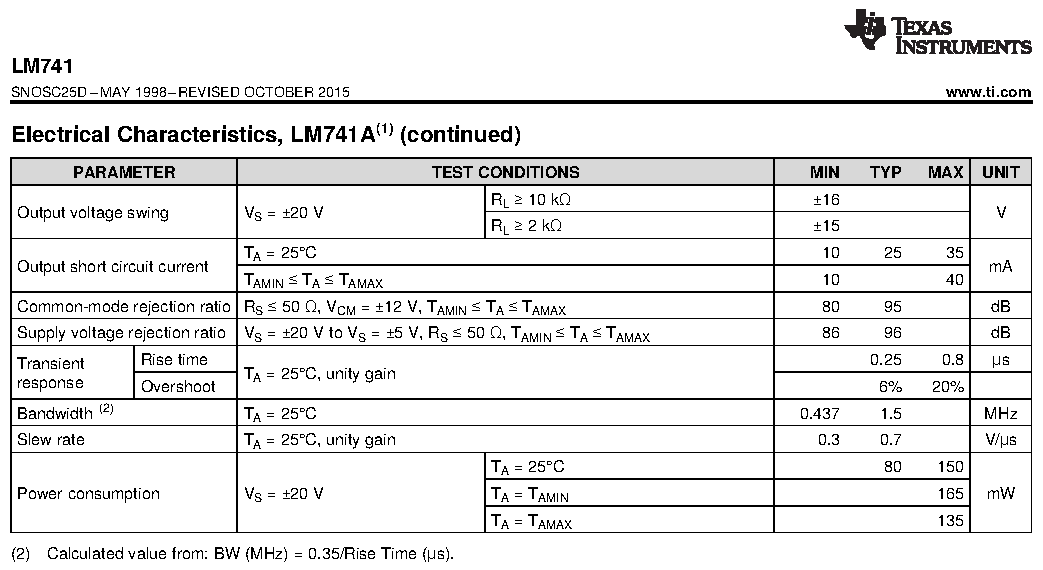
\includegraphics[width=\linewidth]{lm741-gain-bandwidth-crop.pdf}
	\end{center}
}
{
	Le LM741 a un produit gain-bande passante typique de 1.5~MHz.
	Ainsi, pour un gain de 15, la bande passante est de 100~kHz.
}

\Question{\label{q.tension-decalage}%Ex labo 2, 2.7

	En considérant $R_s = 10 k\ohm$, $R_1 = 1 k\ohm$ et $R_2 = 9 k\ohm$~:
	%100k =>10k parce que e0 spécifié pour Rs<=10k
	% \vspace*{3cm}
	% \marginpar{\qrcode[hyperlink,height=0.5in]{https://easyeda.com/editor\#id=UvtGQqemA}}
	% \vspace*{-3cm}

	\begin{center}
		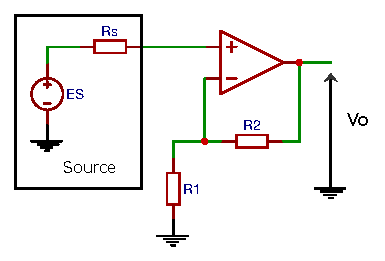
\includegraphics[scale=1.4]{montage-tension-de-decalage.pdf}
	\end{center}

	\begin{enumerate}
		\item Calculez la tension de décalage à la sortie de l'amplificateur, soit $V_o(E_s = 0)$, dans le cas d'un LM741, puis d'un CA3140A.
		Note~: commencez par ajouter la ou les causes de cette tension de décalage sur le montage.
		\item Comparez les deux résultats obtenus. À quoi est due la différence~?
		\paragraph{LM741}
		\begin{center}
			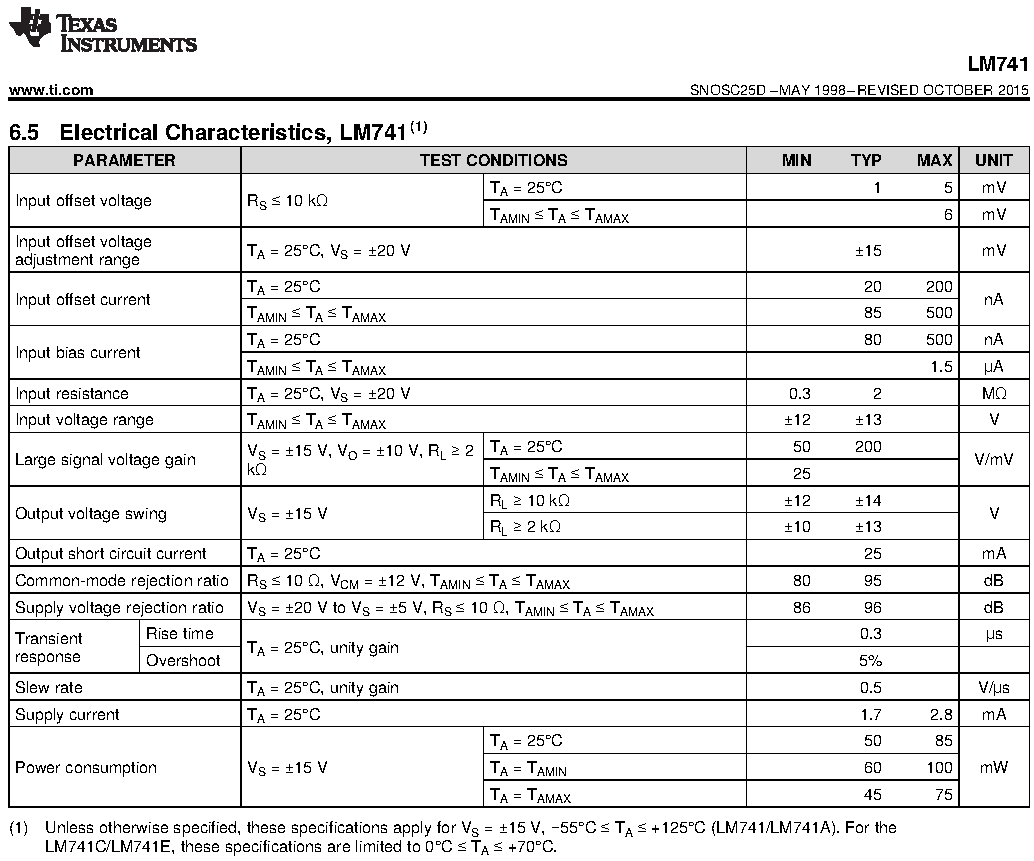
\includegraphics[width=\linewidth]{lm741-offset-voltage-crop.pdf}
		\end{center}

		\paragraph{CA3140A}
		\begin{center}
			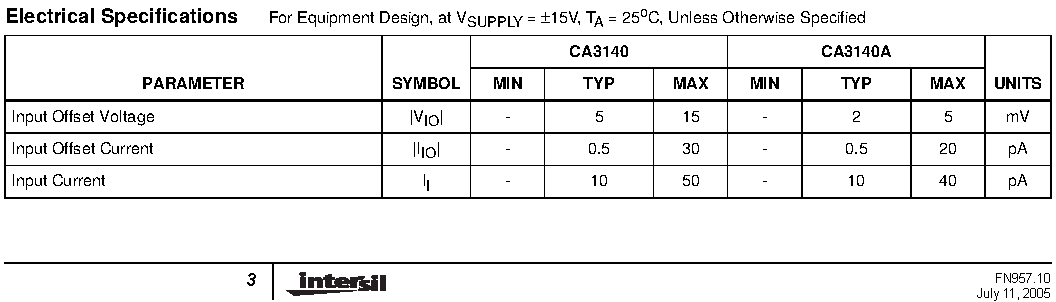
\includegraphics[width=\linewidth]{ca3140-a-offset-voltage-crop.pdf}
		\end{center}


	\end{enumerate}
}
{
	\begin{enumerate}
		\item La tension de décalage en sortie est due aux imperfections de l'ampli-op.
		Ces imperfections sont modélisées pour une source de tension continue $e_0$ à l'entrée non-inverseuse et une source de courant $I_+$ et $I_-$ à chaque entrée.
		\begin{center}
			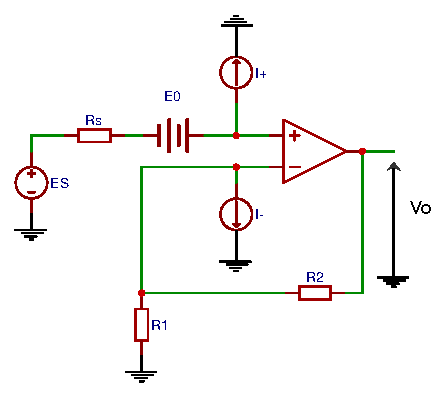
\includegraphics[scale=1.4]{ampli-op-imperfections.pdf}
		\end{center}

		Puisqu'on ignore l'influence de la source «~normale~», le nouveau montage possède trois sources que nous allons étudier par superposition.
		Attention, on a considéré un ampli-op réel (\textit{i.e.} non-idéal) pour mettre en évidence les imperfections de ce dernier.
		Cependant, puisque ces imperfections ont été mise en évidence, qu'elles ont été «~sorties~» de l'ampli-op, on considère à nouveau un ampli-op idéal (et on peut donc utiliser le zéro virtuel).
		\begin{itemize}
			\item Influence de $e_0$~: $V_{out} = (1+\frac{R_2}{R_1})\cdot e_0$.
			\item Influence de $I_+$~: puisqu'on considère encore que l'impédance d'entrée de l'ampli-op est infinie, le courant ne rentre pas dans l'ampli-op et passe entièrement dans $R_s$.
			On a ainsi une tension $-R_s \cdot I_+$ à l'entrée non-inverseuse de l'ampli, donant une sortie $V_{out} = -(1+\frac{R_2}{R_1}) \cdot R_s \cdot I_+$.
			\item Influence de $I_-$~: par le zéro virtuel, $V_+ = V_- = 0$.
			La tension aux bornes de $R_1$ est donc nulle, ce qui implique que tout le courant $I_-$ passe dans $R_2$.
			On a en sortie $V_{out} = R_2 \cdot I_-$.
		\end{itemize}

		En superposant les solutions, on trouve $V_{out} = (1+\frac{R_2}{R_1})\cdot e_0 -(1+\frac{R_2}{R_1}) \cdot R_s \cdot I_+ + R_2 \cdot I_-$.

		$e_0$ se trouve dans les datasheets sous le nom de «~\textit{input offset voltage}~».
		Quant à $I_+$ et $I_-$, ils se retrouvent dans les termes «~\textit{input offset current}~» (courant de décalage) qui vaut $I_+ - I_-$, et «~\textit{input bias current}~» (courant de polarisation) qui vaut $\frac{I_++I_-}{2}$.
		En solvant le système, on peut trouver que $I_+ = i_{bias} + \frac{i_{offset}}{2}$ et $I_- = i_{bias} - \frac{i_{offset}}{2}$.

		Pour le LM741, on trouve $e_0$ = 1~mv, $I_+$ = 90~nA et $I_-$ = 70~nA, ce qui donne $V_{out} = 9.99 mV$.

		Pour le CA3140A, on trouve $e_0$ = 2~mv, $I_+$ = 10.25~pA et $I_-$ = 9.75~pA, ce qui donne $V_{out} = 20 mV$, l'influence des courants d'entrée sur la sortie est négligeable par rapport aux autres tensions du circuit.

		\item La différence est due aux types de transistors utilisés dans chacun des amplis-op.
		Le LM741 fonctionne avec des transistors bipolaires commandés en courant et consomment donc en permanence un certain courant.
		En revanche, le CA3140A fonctionne avec des MOS qui ne demandent presque pas de courant, mais nécessitent une tension de commande légèrement plus élevée.
	\end{enumerate}
}

\Question{%Ex labo 2, 2.8

	Il arrive fréquemment que nous n'ayons pas accès à des alimentations symétriques.
	Par exemple, les lecteurs multimédias portables sont généralement alimentés par des batteries fournissant une tension entre 3~V et 5~V, l'autre borne étant connectée à la masse du système.

	\begin{enumerate}
		\item Tracez la sortie du montage suivant, où $V_{in}$ est une sinusoïde d'amplitude 10~mV et de fréquence 5~kHz.
		Quel problème peut-on observer~?

		\begin{center}
			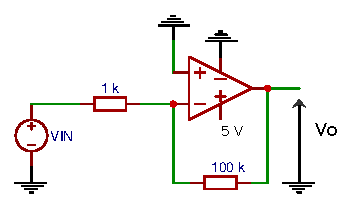
\includegraphics[scale=1.4]{montage-polarisation.pdf}
		\end{center}
		% \vspace*{-2cm}
		% \marginpar{\qrcode[hyperlink,height=0.5in]{https://easyeda.com/editor\#id=6Cp3jIj37}}
		% \vspace*{2cm}

		Pour supprimer ce problème, nous allons polariser le montage, ce qui signifie que nous allons changer la moyenne du signal de sortie au moyen d'un condensateur et d'une tension continue.

		\begin{center}
			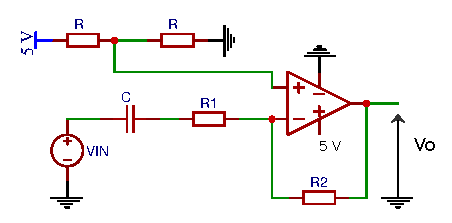
\includegraphics[scale=1.4]{montage-polarisation-complet.pdf}
		\end{center}
		% \vspace*{-2cm}
		% \marginpar{\qrcode[hyperlink,height=0.5in]{https://easyeda.com/editor\#id=i6GXypycA}}
		% \vspace*{2cm}

		\item À l'aide de la superposition, et pour une tension $V_{in}$ à très haute fréquence, expliquez en quoi ce circuit résout le problème.
		Calculez la composante continue de la tension en tous les points du circuit.

		\item Calculez la sortie $V_o = H_1(j\omega_{in}) \cdot V_{in} + H_2(j\omega_{5V}) \cdot 5 V$

		\item Sachant que $V_{in}$ est un signal audio dont la bande passante s'étend de 20~Hz à 20~kHz, dimensionnez R1, R2 et C pour que le gain du montage soit le même que pour le montage non-polarisé dans toute cette bande de fréquence.

		\item Réalisez un filtre RC permettant de supprimer cette composante continue sans déformer la composante alternative.
		Dimensionnez ses composants.
	\end{enumerate}
}
{
	\begin{enumerate}
		\item On obtient une sinusoïde dont les alternances négatives sont ramenées à zéro.
		%\todo[inline]{Trouver un moyen de le faire dans EasyEDA. Pour le moment, on dirait qu'il ne comprend pas où se trouve la masse, il la prend toujours entre les deux bornes d'alimentation.}

		\item Commençons par étudier la source continue seule.
		Le condensateur est alors remplacé par un circuit ouvert.
		On en déduit $V_+ = 2.5V$ et $V_{out} = 2.5 V$, puisque $R_1$ est en circuit ouvert (on a un étage suiveur).

		Passons ensuite à la source alternative seule.
		Cette fois-ci, le condensateur est remplacé par un court-circuit (la fréquence étant considérée comme suffisamment élevée).
		On obtient $V_{out} = -\frac{R_2}{R_1}\cdot V_{in}$.

		La sortie totale sera la somme des sous-circuits~: $V_{out} = 2.5 V - \frac{R_2}{R_1}\cdot V_{in}$.

		La tension de sortie a donc bien été décalée et centrée autour de 2.5~V, il n'y aura donc plus d'écrêtage.

		\item La composante continue ayant une pulsation nulle, on peut l'ignorer pour déterminer le type de filtre.

		En revanche, $H_1(\omega_{in}) = - \frac{R_2}{R_1 + \frac{1}{j\omega_{in}C}} = - \frac{j\omega_{in}C \cdot R_2}{j\omega_{in}R_1C + 1}$. Il s'agit d'un filtre passe-haut.

		\item Puisqu'on veut un gain de -100, on sait que $R_2 = 100 R_1$.

		Ensuite, on veut que le montage soit fonctionnel entre 20~Hz et 20~kHz. Or, le montage étant un passe haut, il faut s'arranger pour que 20~Hz soit déjà considéré comme une haute fréquence.
		Autrement dit, l'impédance du condensateur doit être beaucoup plus faible que $R_1$~: $1 << \omega R_1C \Leftrightarrow \frac{1}{\omega C} << R_1$, avec $\omega = 2 \pi \cdot 20$.

		En prenant arbitrairement $R_1 = 1k\Omega$, on a $R_2 = 100k\Omega$, et donc $C >> 8 \mu F$.
		En pratique, un à deux ordres de grandeur suffisent~: prenons $C = 80 \mu F$.

		\item Il suffit d'ajouter un filtre passe-haut en sortie du montage (pour rappel, il peut s'agir d'un condensateur $C_2$ et d'une résistance $R_3$ en série, en prenant la sortie sur la résistance).

		À nouveau, la fréquence de coupure doit être plus basse que 20~Hz.
		En prenant arbitrairement $R_3 = 100 k\Omega$, on choisira $C_2 = 800 nF$.
	\end{enumerate}
}

% \section{Dimensionnement de circuit à ampli-op}
\Question{%Ex labo 2, 3.1

	\begin{enumerate}
		\item Dimensionnez un étage amplificateur inverseur à ampli-op ayant un gain à vide $A_v = 14 dB$ et une impédance d'entrée $R_{in} \geq 10 k\ohm$

		\item En supposant que l'ampli-op utilisé pour réaliser ce montage est un LM741, déterminez~:
		\begin{itemize}
			\item la bande passante du montage~;
			\item la tension de décalage à la sortie.
		\end{itemize}
	\end{enumerate}
}
{
	\begin{enumerate}
		\item Le gain d'un inverseur est $A = -\frac{R_2}{R_1}$, avec $R_2$ la résistance de rétroaction et $R_1$ la résistance à l'entrée inverseuse.
		Étant donné que 14~dB correspond à un gain de 5, on a $R_2 = 5 R_1$. Notez que le gain en décibel correspond à la valeur absolue du gain «~décimal~».
		Dans le cas du montage inverseur, l'impédance d'entrée correspond à notre $R_1$.
		Puisqu'on veut $R_{in} \geq 10 k\ohm$, on peut prendre $R_1 = 10 k\Omega$ et $R_2 = 50 k\Omega$.

		\item Le produit gain-bande passante («~\textit{gain-bandwidth product}~», ou GBP en anglais) du LM741 étant de 1.5~MHz, la bande passante du montage vaut $\frac{GBP}{|A|} = 300 kHz$.

		La tension de décalage se calcule de la même façon que dans l'exercice~\ref{q.tension-decalage}, à savoir $V_{out} = (1+\frac{R_2}{R_1})\cdot e_0 -(1+\frac{R_2}{R_1}) \cdot R_s \cdot I_+ + R_2 \cdot I_-$.
		Cependant, dans le cas présent, la source $I_+$ est directment connectée à la masse et n'a donc aucune influence.
		On obtient alors $V_{out} = 6\cdot e_0 + R_2 \cdot I_- = 33.5 mV$, puisqu'on a $e_0 = 1mV$ et $I_- = 70nA$.
	\end{enumerate}
}

\Question{%Ex labo 2, 3.2

	On vous demande de réaliser un amplificateur d'entrée pour l'entrée ligne d'une carte son d'ordinateur.
	On vous donne les informations suivantes~:

	\begin{center}
		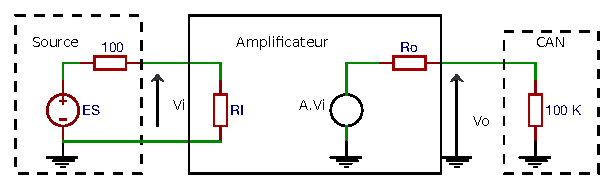
\includegraphics[scale=1.4]{circuit-dimensionnement.pdf}
	\end{center}
		% \vspace*{-2cm}
		% \marginpar{\qrcode[hyperlink,height=0.5in]{https://easyeda.com/editor\#id=o6YcW6iEE}}
		% \vspace*{2cm}

	\begin{itemize}
		\item La source de signal connectée à l'entrée de la carte fournit un signal sans composante continue et dont l'amplitude crête ne dépasse pas 100~mV, et son impédance de sortie est égale à 100~\ohm.%Je passe à 10mV pour qu'on doive utiliser un gain de 100. Comme la bande passante est de 20kHz, il faudrait deux LM741 (GBP 1.5MHz) ou un seul CA3140 (GBP 4.5MHz).
		\item La sortie de l'étage à réaliser est connectée à un convertisseur analogique/numérique (CAN) dont l'impédance d'entrée est égale à 100~k\ohm. La plage de conversion du CAN va de $-1V$  à $+1V$.
		\item Votre montage doit amplifier correctement les signaux entre 20~Hz et 20~kHz.
		\item Vous avez à votre disposition des amplis-op LM741 ou CA3140A.
		Le LM741 coûte 0.54~\EUR/pièce et le CA3140A coûte 1.96~\EUR/pièce.
	\end{itemize}
}
{
	\begin{itemize}
		\item Nous pouvons commencer par établir les contraintes de dimensionnement que nous devons respecter~:
		\begin{itemize}
			\item Impédance d'entrée~: étant donné qu'on travaille en tension, l'adaptation d'impédance doit se faire en tension à l'entrée de l'amplificateur~: $R_i >> 100 \Omega$.
			\item Gain~: la valeur de crête du signal d'entrée est inférieure ou égale à 100~mV, et la valeur de crête admissible par le CAN est de 1~V. Le gain maximal vaut donc $A = \frac{1V}{100mV} = 10$.
			\item Impédance de sortie~: on adapte à nouveau en tension, donc $R_o << 100 k\Omega$.
		\end{itemize}

		Sur base de ces critères, choisissons l'un des deux montages amplificateurs classiques (inverseur et non-inverseur).
		Pour faire ce choix, il faut examiner les différences essentielles entre ces deux montages.\\

		\begin{center}
			\begin{tabularx}{.9\textwidth}{l|X|X}
			& Inverseur & Non-inverseur \\ \hline
			Impédance d'entrée & Égale à la résistance connectée à l'entrée inverseuse. & Quasi-infinie, l'adaptation d'impédance en tension est donc toujours effectuée. \\ \hline
			Signe du gain & Inverse le signal. Lorsqu'il y a une composante continue, ce peut être gênant, mais s'il ne s'agit que d'un signal périodique alternatif, ça revient simplement à un déphasage de 180°. & Positif. \\ \hline
			Valeur du gain & Au choix. & Ne peut être inférieur à 1. \\
			\end{tabularx}
		\end{center}

		En conclusion, étant donné qu'on a un signal purement sinusoïdal et qu'on veut un gain supérieur à 1, les deux montages sont acceptables.
		On choisira en général le montage non-inverseur pour son impédance d'entrée et la conservation du signe du signal.

		Il reste à vérifier qu'un seul étage est suffisant au vu du produit gain-bande passante (GBP) de chacun des modèles.
		Étant donné qu'il nous faut un gain de 10 pour une bande passante de 20~kHz, le GBP du LM741 et du CA3140A (respectivement 1.5~MHz et 4.5~MHz) est suffisant pour qu'un seul étage fasse l'affaire.

		On peut finalement s'en sortir avec un seul montage non-inverseur comprenant une résistance de rétroaction de 90~k\ohm\ et une résistance sur l'entrée inverseuse de 10~k\ohm.
	\end{itemize}
}

\Question{%Ex labo 2, janvier 2003

	On désire amplifier un signal dont la bande passante s'étend de 2~kHz à 2~MHz.
	Ce signal est représenté par une source composée d'une f.e.m. sinusoïdale $V_{in}$ de 10~mV et d'une impédance de sortie de 50~\ohm.
		% \vspace*{2.5cm}
		% \marginpar{\qrcode[hyperlink,height=0.5in]{https://easyeda.com/editor\#id=G9yeSbAQn}}
		% \vspace*{-2.5cm}

	\begin{center}
		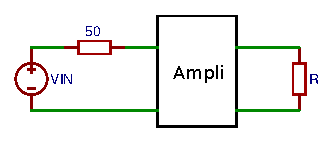
\includegraphics[scale=1.4]{dimensionnement-janvier-2003.pdf}
	\end{center}

	On désire obtenir à la sortie du bloc amplificateur, aux bornes de la charge $R$, un signal~:
	\begin{itemize}
		\item d'amplitude réglable, comprise entre 5~mV et 4~V au choix de l'utilisateur~;
		\item non déphasé par rapport au signal d'entrée.
	\end{itemize}

	\begin{enumerate}
		\item En supposant que l'impédance de charge $R$ vaut 10~k\ohm, proposez et dimensionnez un montage pour le bloc amplificateur.
		Justifiez chaque étape de votre raisonnement et donnez un schéma final complet de votre montage amplificateur.

		\item En supposant maintenant que la résistance de charge $R_c$ vaut 4~\ohm, comment faut-il modifier le montage et pourquoi~?
	\end{enumerate}

	Remarques~:
	\begin{itemize}
		\item Vous disposez de trois types d'amplis-op dont les caractéristiques sont données dans le tableau ci-dessous.
		Si plusieurs solutions sont possibles, utilisez toujours la solution la moins coûteuse.
		\item Pour chacune des questions ci-dessus, justifiez brièvement chaque étape de votre raisonnement.
	\end{itemize}

	\begin{center}
		\begin{tabular}{|c|c|c|c|c|c|} \hline
		Type & $V_{DD}$ & $I_{out, max}$ [mA] & $A.B_w$ [MHz] & Slew-rate [V/µs] & Prix [\EUR] \\ \hline
		AD8129 & 3~V à 12~V & 40 & 200 & 1070 & 3.65 \\ \hline %spec à +/-12V
		OPA549 & 8~V à 60~V & 8000 & 0.9 & 100 & 21.31 \\ \hline
		OPA132 & 4.5~V à 36~V & 40 & 8 & 20 & 3.97 \\ \hline
		\end{tabular}
	\end{center}
}
{
	\begin{enumerate}
		\item Établissons tout d'abord les contraintes de dimensionnement que nous devons respecter~:
		\begin{itemize}
			\item impédance d'entrée~: $R_i >> 50 \Omega$. Les deux types de montages sont possible.
			\item gain~: $0.5 \leq A \leq 400$. Étant donné le gain inférieur à 1, il faut au moins un étage inverseur.
			\item impédance de sortie~: $R_o << 10 k\Omega$. Les deux types de montages sont possible.
			\item déphasage~: nul. Il faut un nombre pair d'inverseurs.
		\end{itemize}

		Le montage final comprendra au moins deux étages inverseurs.

		Déterminons le gain maximum permit par chacun des amplis-op pour la bande passante requise~:

		\begin{center}
			\begin{tabular}{l|c|c|c}
			AOP & AD8129 & OPA549 & OPA132 \\ \hline
			Gain & 100 & 0.45 & 4 \\
			\end{tabular}
		\end{center}

		On peut immédiatement écarter l'OPA549, il est non seulement moins bon, mais aussi plus cher.
		La solution la moins chère pour obtenir un gain total de 400 est d'utiliser deux étages inverseurs à base de AD8129.

		Cependant, si la résistance de charge vaut 4~\ohm, l'adaptation d'impédance à la sortie est certes respectée (en supposant une résistance nulle à la sortie de l'ampli-op), mais l'ampli-op doit pouvoir fournir un courant dont l'amplitude de crête est de $\frac{4V}{4\Omega} = 1 A$.
		Or le ampli-op sélectionné ne peut fournir que 40~mA.
		Il faut donc ajouter un troisième étage de gain 1 (montage suiveur de tension) qui servira à fournir de la puissance à la charge.
		On peut alors utiliser l'OPA549 qui peut fournir jusqu'à 8~A.
		C'est cette caractéristique qui justifie son prix.

		Le montage final comprend donc deux étages inverseurs (l'un à base d'AD8129, l'autre d'OPA132) et un étage suiveur de sortie (à base d'OPA549).
	\end{enumerate}
}

% \Question{

 	% \begin{center}
% 		\begin{tabular}{|c|c|c|} \hline
% 		Modèle & GBP [MHz] & \EUR/pièce \\ \hline
% 		TL081CN & 4 & 1.67 \\ \hline
% 		TLE2061 & 1.8 & 1.88 \\ \hline
% 		LM741 & 1.5 & 0.54 \\ \hline
% 		CA3140A & 4.5 & 1.96 \\ \hline
% 		\end{tabular}
% 	\end{center}
% }
% {}





\end{document}
